\begin{figure}[t]
\begin{center}
\begin{small}
\begin{sc}
\begin{tabular}{ccc}
Image & Target & Result \\
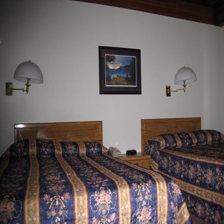
\includegraphics[width=\medimg]{figures_sup/seg_ade/0/input.png} & 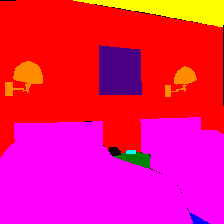
\includegraphics[width=\medimg]{figures_sup/seg_ade/0/target.png} & 
\includegraphics[width=\medimg]{figures_sup/seg_ade/0/ours.png} \\

\includegraphics[width=\medimg]{figures_sup/seg_ade/1/input.png} & 
\includegraphics[width=\medimg]{figures_sup/seg_ade/1/target.png} & 
\includegraphics[width=\medimg]{figures_sup/seg_ade/1/ours.png} \\

\includegraphics[width=\medimg]{figures_sup/seg_ade/3/input.png} & 
\includegraphics[width=\medimg]{figures_sup/seg_ade/3/target.png} & 
\includegraphics[width=\medimg]{figures_sup/seg_ade/3/ours.png} \\

\includegraphics[width=\medimg]{figures_sup/seg_ade/4/input.png} & 
\includegraphics[width=\medimg]{figures_sup/seg_ade/4/target.png} & 
\includegraphics[width=\medimg]{figures_sup/seg_ade/4/ours.png} \\

\includegraphics[width=\medimg]{figures_sup/seg_ade/5/input.png} & 
\includegraphics[width=\medimg]{figures_sup/seg_ade/5/target.png} & 
\includegraphics[width=\medimg]{figures_sup/seg_ade/5/ours.png} \\

\includegraphics[width=\medimg]{figures_sup/seg_ade/6/input.png} & 
\includegraphics[width=\medimg]{figures_sup/seg_ade/6/target.png} & 
\includegraphics[width=\medimg]{figures_sup/seg_ade/6/ours.png}
\end{tabular}
\end{sc}
\end{small}
\end{center}
\vskip -0.1in
\caption{\textbf{Image segmentation on ADE20K:} Figure shows the qualitative results of the image segmentation task. Image size is $224\times224$ and $12\times48^2$ adaptive glimpses are used.}
\end{figure}